%%----------------------------------------------------------------------------
%% Onderzoekstechnieken: Toetsingsprocedures
%%----------------------------------------------------------------------------

\documentclass[aspectratio=169]{beamer}

%==============================================================================
% Aanloop
%==============================================================================

%---------- Vormgeving --------------------------------------------------------

\usetheme{hogent}

\usecolortheme{hgwhite} % witte achtergrond, zwarte tekst

\usepackage{graphicx,multicol}
\usepackage{comment,enumerate,hyperref}
\usepackage{amsmath,amsfonts,amssymb}
\usepackage[dutch]{babel}
\usepackage{multirow}
\usepackage{eurosym}
\usepackage{listings}
\usepackage{textcomp}
\usepackage{framed}
\usepackage{wrapfig}
\usepackage{tabu} %needed for \tabulinesep
\usepackage{wrapfig}
\usepackage{pgf-pie}
\usepackage{pgfplots}
\usepackage{booktabs}
\usepackage{pgfplotstable}
\usepackage{changepage}
\usepackage{ulem} % for \sout{text} (strikethrough)
\usepackage{fancyvrb} % for \begin{Verbatim} (LaTeX controls within verbatim)

%---------- Configuratie ------------------------------------------------------

\pgfplotsset{compat=1.16}
\usetikzlibrary{arrows,shapes,backgrounds,positioning,shadows}
\usetikzlibrary{pgfplots.statistics}

%---------- Commando-definities -----------------------------------------------

\newcommand{\tabitem}{~~\llap{\textbullet}~~}
\newcommand{\alertbox}[2][hgblue]{%
  \setbeamercolor{alertbox}{bg=#1,fg=white}
  \begin{beamercolorbox}[sep=2pt,center]{alertbox}
    \textbf{#2}
  \end{beamercolorbox}
}
\pgfmathdeclarefunction{gauss}{2}{%
  \pgfmathparse{1/(#2*sqrt(2*pi))*exp(-((x-#1)^2)/(2*#2^2))}%
}

%---------- Info over de presentatie ------------------------------------------

\title{Hst 5. Toetsingsprocedures}
\subtitle{Onderzoekstechnieken}
\author{Jens Buysse \and Wim {De Bruyn} \and Pieter-Jan Maenhout \and Bert {Van Vreckem}}
\date{AJ 2019-2020}

%==============================================================================
% Inhoud presentatie
%==============================================================================

\begin{document}

\begin{frame}
  \maketitle
\end{frame}

\begin{frame}
  \frametitle{What's on the menu today?}
  
  \tableofcontents
\end{frame}

\begin{frame}
  \frametitle{What's on the menu today?}
  
  \tableofcontents
\end{frame}

\begin{frame}
  \frametitle{Leerdoelen}
  
  \begin{itemize}
    \item Statistische toetsen: begrippen
    \item Procedure van statistische toetsen
    \item $z$- en $t$-toets toepassen
  \end{itemize}
\end{frame}


\section{Toetsen van hypothesen}

\begin{frame}
  \frametitle{De statistische toets voor een hypothese}
  
  \begin{description}
    \item[Hypothese] Idee waarvan nog bewezen moet worden dat het juist is: uitspraak over numerieke waarde van een populatieparameter
    \item[Hypothesetoets] controle van een uitspraak over de waarden van één of meerdere populatieparameters
    \item[Nulhypothese ($H_0$)] Deze hypothese proberen we te ontkrachten door redenering in het ongerijmde
    \item[Alternatieve hypothese ($H_1$, $H_a$)] Deze hypothese willen we aantonen
  \end{description}
\end{frame}

\begin{frame}
  \frametitle{Elementen bij toetsingsprocedure}
  
  \begin{description}
    \item[Toetsingsgrootheid] De variabele die berekend wordt uit de steekproef (ook: teststatistiek)
    \item[Aanvaardingsgebied] Het gebied van waarden die de nulhypothese \alert{ondersteunt}
    \item[Kritieke of Verwerpingsgebied] Het gebied van waarden die de nulhypothese \alert{verwerpt}
    \item[Significantieniveau] De kans dat $H_0$ \alert{onterecht} verworpen wordt
  \end{description}
\end{frame}

\section{Werkwijze}

\begin{frame}
  \frametitle{Werkwijze}
  
  \begin{enumerate}
    \item Bepalen van de hypothesen ($H_0$ en $H_1$)
    \item Vastlegen significantieniveau ($\alpha$)
    \item Toetsingsgrootheid berekenen
    \item Het kritieke gebied of de overschrijdingskans bepalen
    \item Conclusies trekken
  \end{enumerate}
\end{frame}

\begin{frame}[plain]
  \frametitle{Hypothesen over superhelden}
  \centering
  
\includegraphics[height=.85\textheight]{les5-heroes}
\end{frame}

\begin{frame}
  \frametitle{Een superheld redt 3.3 mensen per dag}
  
  \begin{columns}
    \column{.5\textwidth}
    \centering
    
\includegraphics[width=3cm]{les5-gered1}
    
    
\includegraphics[width=3cm]{les5-gered2}
    \column{.5\textwidth}
    \centering
    
\includegraphics[width=3cm]{les5-gered3}
    
    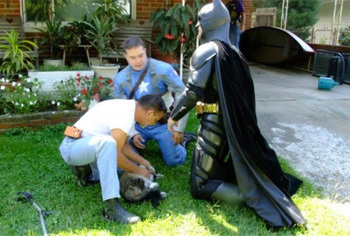
\includegraphics[width=3cm]{les5-gered4}
  \end{columns}
  
  \vfill
  \centering
  \small{Bron: \url{http://www.cracked.com/quick-fixes/4-people-who-saved-day-while-dressed-as-superheroes/}}
\end{frame}

\begin{frame}
  Stel, in een periode van 30 dagen werden er gemiddeld $3,483$ mensen per dag gered ($\overline{x}=3,483$, $n=30$)
  \vfill
  \begin{enumerate}
    \item Hypothese: $H_0: \mu = 3,3$; $H_1: \mu > 3,3$
    \item Significantieniveau: $\alpha = 0,05$
    \item Toetsingsgrootheid: $\overline{x} = 3,483$
  \end{enumerate}
  \vfill
  Populatiestandaardafwijking (verondersteld gekend): $\sigma = 0,55$
\end{frame}

\begin{frame}
  \frametitle{Berekenen toetsingsgrootheid}
  
  \bigskip
  
  Uit centrale limietstelling volgt: $M \sim Nor(\mu = 3,3; \sigma = \frac{0,55}{\sqrt{30}}=0,1)$
  
  \centering
  \begin{tikzpicture}[scale=.8]
  \begin{axis}[domain=3.0:3.6, ymax=4.2, samples=100, enlargelimits=false ]
  \addplot [very thick,smooth,draw=hgblue] {gauss(3.3, 0.10041580220928045413)};
  \node [coordinate, pin={$\overline{x}= 3.483$}] at (axis cs: 3.483, 0){};
  \end{axis}
  \end{tikzpicture}
\end{frame}

\section{Overschrijdingskans}

\begin{frame}
  \frametitle{Overschrijdingskans}
  \alertbox{De \textcolor{hgyellow}{p-waarde} is de kans, indien de nulhypothese waar is, om een waarde te verkrijgen voor de toetsingsgrootheid die minstens even extreem is als de geobserveerde waarde.}
  
  \begin{itemize}
    \item $p$-waarde $< \alpha \Rightarrow$ $H_{0}$ verwerpen: de gevonden waarde voor $\overline{x}$ is te extreem;
    \item $p$-waarde $\geq \alpha \Rightarrow$ $H_{0}$ niet verwerpen: de gevonden waarde voor $\overline{x}$ kan nog verklaard worden door toeval.
  \end{itemize}
\end{frame}

\begin{frame}
  \frametitle{Overschrijdingskans}
  
  \bigskip
  
  \centering
  \begin{tikzpicture}[scale=0.6]
  \begin{axis}[domain=-3.5:3.5, ymax=0.42, samples=100, enlargelimits=false, clip=false ]
  \addplot [smooth, fill=black!20, domain=1.822:3.5] {gauss(0,1)} \closedcycle;
  \addplot [very thick,smooth,draw=hgblue] {gauss(0, 1)};
  \node  at (axis cs: 1.822, -.04){\small 1.822};
  \draw [-latex](axis cs:2.1,0.02) -- (axis cs:2.35,0.06);
  \node [text width=0.5cm] at (axis cs: 2.5, .095){$p= 0,0344$};
  \end{axis}
  \end{tikzpicture}
  
  \[ P(M > 3,483) = P \left(Z> \frac{3,483 - 3,3}{\frac{\sigma}{\sqrt{n}}}\right) = P (Z > 1,822) = 0,0344 \]
\end{frame}

\section{Kritieke gebied}

\begin{frame}
  \frametitle{Kritieke gebied}
  
  \bigskip
  
  \alertbox{Het \textcolor{hgyellow}{kritieke gebied} is de verzameling van alle waarden voor de toetsingsgrootheid waarbij de nulhypothese kan verworpen worden.}
  
  We zoeken een grenswaarde $g$ waarvoor geldt:
  \[ P(M > g) = \alpha \]
  
  Bepaal $z_\alpha$ waarvoor geldt:
  \[ P(Z > z_\alpha) = \alpha \Rightarrow g = \mu + z_\alpha . \frac{\sigma}{\sqrt{n}} \]
  
  \begin{itemize}
    \item Links van $g$: aanvaardingsgebied ($H_0$ niet verwerpen)
    \item Rechts van $g$: kritieke gebied ($H_0$ wel verwerpen)
  \end{itemize}
  
\end{frame}


\begin{frame}
  \frametitle{Kritieke gebied}
  
  \centering
  \begin{tikzpicture}[scale=.9]
  \begin{axis}[domain=-3.5:3.5, ymax=0.42, samples=100, enlargelimits=false, clip=false ]
  \draw [-](axis cs:1.645,-0.03) -- (axis cs:1.645,0.06);
  \addplot [smooth, fill=black!20, domain=1.645:3.5] {gauss(0,1)} \closedcycle;
  \addplot [very thick,smooth,draw=hgblue] {gauss(0, 1)};
  \node [text width=0.8cm] at (axis cs: 1.645, -.06){$z_{\alpha}= 1.645$};
  \draw [-latex](axis cs:2.1,0.02) -- (axis cs:2.35,0.06);
  \node [text width=0.5cm] at (axis cs: 2.5, .095){$\alpha= 0.05$};
  \end{axis}
  \end{tikzpicture}
  
  significantieniveau $\alpha = 0.05$ $\Rightarrow$ grenswaarde $z_{\alpha}$=1.645\\
  ($z_{\alpha} = $\texttt{qnorm(0.95)})
  
\end{frame}

\begin{frame}
  \frametitle{Linkszijdig toetsen}
  
  Wat zou je in de verg.  moeten veranderen opdat je de correcte kritieke waarde zou berekenen?
  \pause
  Antwoord:
  \[g = \mu \alert{-} z \times \frac{\sigma}{\sqrt{n}} \]
  want
  \[ P(M < g) = P\left(Z < \frac{g - \mu}{\frac{\sigma}{\sqrt{n}}}\right) = 0.05 \]
  
\end{frame}

\begin{frame}
  \frametitle{Linkszijdig toetsen}
  Wegens de symmetrieregel kunnen we zeggen
  \[ P\left(Z > - \left( \frac{g - \mu}{\frac{\sigma}{\sqrt{n}}} \right) \right) = 0.05 \]
  
  De z-waarde die ermee overeen komt is 1.645 dus hebben we
  
  \begin{align*}
  z = \frac{-g + \mu}{\frac{\sigma}{\sqrt{n}}} &\Leftrightarrow -g = \frac{\sigma}{\sqrt{n}} z - \mu \\
  & \Leftrightarrow g = \mu - z \frac{\sigma}{\sqrt{n}}
  \end{align*}
  
\end{frame}

\begin{frame}
  \frametitle{Tweezijdig toetsen}
  Soms kan het ook zijn dat er tweezijdig moet getoetst worden. Er moeten dan twee kritieke grenswaarden berekend worden namelijk de linker- en de rechter grenswaarden.
  
  \begin{equation}
  g = \mu \pm z \times \frac{\sigma}{\sqrt{n}}
  \label{eq:kritiekeGrenswaarde}
  \end{equation}
\end{frame}

\begin{frame}[plain]
  \frametitle{Samenvatting}
  
  \begin{table}
    \centering
    \begin{tabular}{l|ccc}
      \toprule
      Doel              & \multicolumn{3}{l}{\parbox{.7\textwidth}{Test op gemiddelde waarde $\mu$ van de populatie aan de hand van een steekproef van $n$ onafhankelijke steekproefwaarden}} \\
      \midrule
      Voorwaarde        & \multicolumn{3}{l}{\parbox{.7\textwidth}{De populatie is willekeurig verdeeld, $n$ voldoende groot}} \\
      \midrule
      Type test         & Tweezijdig           & Eenzijdig links & Eenzijdig rechts \\
      \midrule
      $H_{0}$           & $\mu = \mu_{0}$      & $\mu = \mu_{0}$ & $\mu = \mu_{0}$  \\
      $H_{1}$           & $\mu \neq \mu_{0}$   & $\mu < \mu_{0}$ & $\mu > \mu_{0}$  \\
      Verwerpingsgebied & $\left|z\right| > g$ & $z< -g $        & $z>g$            \\
      Teststatistiek    & \multicolumn{3}{c}{$z = \frac{\overline{x} - \mu_{0}}{\frac{\sigma}{\sqrt{n}}}$} \\
      \bottomrule
    \end{tabular}
    \caption{Samenvatting mogelijke toetsen}
    \label{tab:toetsingsprocedures}
  \end{table}
\end{frame}

\section{Voorbeelden}

\begin{frame}
  \frametitle{Voorbeeld 1}
  Bij een aselecte steekproef van 50 waarnemingen vinden we volgende grootheden: gemiddelde $\overline{x} = 25$ en standaardafwijking s = $\sqrt{55} = 7.41$
  We willen weten of er reden is om aan te nemen dat gemiddelde van de populatie kleiner is dan 27.
  
\end{frame}

\begin{frame}
  \frametitle{Voorbeeld 1}
  
  \begin{description}
    \item[1] Bepalen van de hypothesen
    
    $H_{0} : \mu = 27$ en $H_{1}: \mu < 27$.
    
    \item[2] Vastleggen significantieniveau
    
    $\alpha = 0.05$ en $n=50$
    
    \item[3] Toetsingsgrootheiden \& waarde: steekproefgemiddelde $\overline{x} = 25$
    
    
  \end{description}
\end{frame}

\begin{frame}
  \frametitle{Voorbeeld 1 (vervolg)}
  
  \begin{description}
    \item[4a] Overschrijdingskans
    
    Volgens de centrale limietstelling geldt:
    
    \[ M \sim Nor(\mu = 27, \frac{\sigma}{\sqrt{n}}) \]
    \[ z = \frac{\overline{x} - \mu}{\frac{\sigma}{\sqrt{n}}} = \frac{25-27}{\sqrt\frac{55}{50}} \approx -1.91\]
    
    We vinden dus een overschrijdingskans van het gemiddelde $0.0281$.
    
    
    Bij een significantieniveau van 0.05 mogen we $H_{0}$ verwerpen.
  \end{description}
  
\end{frame}

\begin{frame}
  \frametitle{Voorbeeld 1 (vervolg)}
  
  \begin{description}
    
    \item[4b] Bereken en teken kritiek gebied
    
    \begin{align*}
    g &= \mu - z \times \frac{\sigma}{\sqrt{n}} \\
    &= 27 - 1.645 \times \sqrt{\frac{\sigma}{n}} \\
    &= 25.27470944
    \end{align*}
    
    We vinden dus dat $\overline{x} < g$ en dus kunnen we $H_{0}$ verwerpen.
  \end{description}
\end{frame}

\begin{frame}
  \frametitle{Voorbeeld 1 (vervolg)}
  
  \bigskip
  \centering
  \begin{tikzpicture}
  \begin{axis}[domain=24:30, samples=100, enlargelimits=false, clip=false ]
  \addplot [smooth, fill=cyan!20, domain=24:25.27] {gauss(27,1.048808848)} \closedcycle;
  \addplot [very thick,smooth,draw=hgblue] {gauss(27, 1.048808848)};
  \node  at (axis cs: 25.27, -.04){\small 25.27};
  \end{axis}
  \end{tikzpicture}
\end{frame}

\begin{frame}
  \frametitle{Voorbeeld 1 (vervolg)}
  
  \begin{description}
    
    \item[5] Conclusie
    
    We besluiten op basis van de steekproef dat $\mu < 27$ met een significantieniveau van $0,05$
  \end{description}
\end{frame}


\begin{frame}
  \frametitle{Voorbeeld 2}
  In een onderzoek naar het kleingeld dat in de zakken van  van  onze superhelden zit, wordt er van uit gegaan dat ze gemiddeld \euro{25} op zak hebben. We gaan ervan uit dat we een gekende spreiding van $\sigma = 7$ hebben. Verder zijn de gegevens van de aselecte steekproef van omvang $n=64$ beschikbaar met gemiddeld zakgeld $\overline{x}$ van \euro{23}. Neem als significantieniveau $\alpha = 0.05$.
\end{frame}

\begin{frame}
  \frametitle{Voorbeeld 2}
  
  \begin{description}
    \item[1] Bepalen van de hypothesen
    
    $H_{0} : \mu = 25$ en $H_{1}: \mu \neq 25$
    
    \item[2] Vastleggen significantieniveau
    
    $\alpha = 0.05$ en $n=64$.
    
    \item[3] Toetsingsgrootheden \& waarde: $\overline{x} = 23$
  \end{description}
  
\end{frame}

\begin{frame}
  \frametitle{Voorbeeld 2 (vervolg)}
  
  \begin{description}
    \item[4b] Bereken kritieke gebied
    
    \[ g_{1} = \mu - z \times \frac{\sigma}{\sqrt{n}} = 23.28 \]
    \[ g_{2} = \mu + z \times \frac{\sigma}{\sqrt{n}} = 26.72 \]
    
    We vinden dat $\overline{x}$ in het kritieke gebied ligt (want $23 < 23.28$) dus mogen we $H_{0}$ verwerpen.
    \item[5] We kunnen op basis van deze steekproef besluiten dat de superhelden \textit{minder} dan \EUR{25} op zak hebben, met een significantieniveau van 5\%
  \end{description}
\end{frame}

\section{De $t$-toets}

\begin{frame}
  \frametitle{Veronderstellingen $z$-toets}
  
  
  \begin{itemize}
    \item De steekproef moet aselect zijn
    \item De steekproef moet voldoende groot zijn ($n \ge 30$)
    \item De variatie van de toetsingsgrootheid moet normaal verdeeld zijn
    \item We veronderstellen dat de standaardafwijking van de populatie, $\sigma$, gekend is
  \end{itemize}
  
  Als deze veronderstellingen niet gelden, mag je de $z$-toets niet gebruiken!
\end{frame}

\begin{frame}
  \frametitle{De $t$-toets}
  
  Bepalen kritieke grenswaarde:
  
  \[ g = \mu \pm t \times \frac{s}{\sqrt{n}} \]
  
  \begin{itemize}
    \item $t$-waarde wordt afgeleid uit de Student-$t$ verdeling, hangt af van aantal \textit{vrijheidsgraden}, $n-1$
    \item Op te zoeken in $t$-tabel of met R-functie \texttt{pt}
    \item Procedure hypothesetoets is verder identiek aan $z$-toets
  \end{itemize}
  
\end{frame}

\section{Fouten in hypothesetoetsen}

\begin{frame}
  \frametitle{Fouten in hypothesetoetsen}
  
  \begin{table}
    \centering
    \resizebox{\textwidth}{!}{%
      \begin{tabular}{@{}l|cc@{}}
        \toprule
        & \multicolumn{2}{c}{\textbf{Realiteit (onbekend)}} \\
        \textbf{Conclusie toets}          & \textbf{$H_{0}$ correct} & \textbf{$H_{1}$ correct}     \\
        \midrule
        \textbf{$H_{0}$ geaccepteerd}& Juist                    & Fout van type II \\
        \textbf{$H_{0}$ verworpen}   & Fout van type I          & Juist            \\
        \bottomrule
      \end{tabular}
    }
    \label{tab:hypfouten}
  \end{table}
  
  P(type I error) = $\alpha$ (= significantieniveau)
  
  P(type II error) = $\beta$
  
  $\beta$ berekenen is \textbf{\textit{niet}} triviaal, maar als $\alpha \searrow$ dan $\beta \nearrow$ 
\end{frame}

\end{document}